\documentclass[12pt,a4paper]{report}

% ================= PACKAGES =================
\usepackage[utf8]{inputenc}
\usepackage[T1]{fontenc}
\usepackage[french]{babel}
\usepackage{graphicx}
\usepackage{amsmath,amssymb}
\usepackage{geometry}
\usepackage[dvipsnames,table]{xcolor}
\usepackage[hidelinks,colorlinks=true,
            linkcolor=MidnightBlue,
            citecolor=ForestGreen,
            urlcolor=BrickRed]{hyperref}
\usepackage{float}
\usepackage{caption}
\usepackage{subcaption}
\usepackage{titlesec}
\usepackage{etoolbox}
\usepackage{booktabs}
\usepackage{tabularx}
\usepackage{longtable}
\usepackage{multirow}
\usepackage{array}
\usepackage{setspace}
\onehalfspacing
\usepackage[expansion=false]{microtype}
\usepackage{fancyhdr}
\usepackage{listings}
\usepackage{enumitem}
\usepackage{tocbibind}
\usepackage{acronym}
\usepackage{graphbox}

% Référence des figures dans figures/ (images PNG de contenu)
\graphicspath{{images/}}


\geometry{
  left=2.2cm,
  right=2.2cm,
  top=2.2cm,
  bottom=2.5cm
}


% ================= CHAPTER FORMAT =================
\titleformat{\chapter}
{\normalfont\Large\bfseries}
{Chapitre \thechapter\ :}
{1em}
{}
\titlespacing*{\chapter}{0pt}{6pt}{18pt}
% Chapitres : saut de page automatique standard (comportement par défaut de \chapter)


% ── Section / subsection : enchaînement continu (aucun saut de page forcé) ──
\titleformat{\section}{\large\bfseries\color{MidnightBlue}}{{\thesection}}{0.7em}{}[\titlerule]
\titleformat{\subsection}{\normalsize\bfseries}{{\thesubsection}}{0.6em}{}
\titlespacing{\section}{0pt}{16pt}{6pt}
\titlespacing{\subsection}{0pt}{10pt}{4pt}


% ── En-têtes ──
\pagestyle{fancy}\fancyhf{}
\setlength{\headheight}{14pt}
\fancyhead[L]{\small\textit{Rapport de stage --- ARSII}}
\fancyhead[R]{\small\textit{Gestion des contacts R\&I Europe--Afrique}}
\fancyfoot[C]{\thepage}
\renewcommand{\headrulewidth}{0.4pt}


% ── Couleurs et listings ──
\definecolor{mainblue}{RGB}{30,80,155}
\definecolor{darkgreen}{RGB}{0,100,0}
\definecolor{codegreen}{rgb}{0.25,0.49,0.48}
\definecolor{codegray}{rgb}{0.5,0.5,0.5}
\definecolor{colorpurple}{rgb}{0.58,0,0.82}
\definecolor{backcolour}{rgb}{0.95,0.95,0.96}
\definecolor{lightgray}{RGB}{245,245,245}


\lstdefinestyle{mystyle}{
    backgroundcolor=\color{backcolour},
    commentstyle=\color{codegreen},
    keywordstyle=\color{colorpurple}\bfseries,
    numberstyle=\tiny\color{codegray},
    stringstyle=\color{codegreen},
    basicstyle=\ttfamily\small,
    breakatwhitespace=false,
    breaklines=true,
    captionpos=b,
    keepspaces=true,
    numbers=left,
    numbersep=5pt,
    showspaces=false,
    showstringspaces=false,
    showtabs=false,
    tabsize=2,
    frame=single,
    rulecolor=\color{codegray!30}
}
\lstset{style=mystyle}


\hypersetup{
    pdftitle={Rapport de stage - Plateforme de gestion des contacts R et I Europe-Afrique - ARSII},
    pdfauthor={Moedem Errachi}
}

% ── Page liminaires : comptage de pages neutralisé ──
\pagenumbering{gobble}

\begin{document}

% ══════════════════════════════════════════════
% PAGE DE GARDE
% ══════════════════════════════════════════════
\begin{titlepage}
    \centering

    % Logos côte à côte
    \begin{minipage}{0.45\textwidth}
        \begin{flushleft}
            
\includegraphics[height=2.2cm]{images/logo_universite.png}
        \end{flushleft}
    \end{minipage}
    \begin{minipage}{0.45\textwidth}
        \begin{flushright}
            
\includegraphics[height=2.2cm]{images/logo_arsii.png}
        \end{flushright}
    \end{minipage}

    \vspace{0.8cm}

    % Institution & Formation
    {\large \textbf{Faculté des Sciences de Tunis}}\\[0.2cm]
    {\normalsize Cycle Ingénieur --- Génie Logiciel}\\[0.6cm]

    {\small \textit{En collaboration avec}}\\[0.1cm]
    {\large \textbf{ARSII}}\\
    {\small \textit{Association de Recherche Scientifique et Innovation en Informatique}}\\[1.2cm]

    % Intitulé du document
    {\Large \textbf{Rapport de stage}}\\[0.2cm]
    {\large \textit{Développement d'une plateforme de gestion des contacts}}\\[0.4cm]

    % Titre principal encadré par des lignes
    \rule{\linewidth}{0.5mm} \\[0.4cm]
    {\huge \bfseries Plateforme de gestion des contacts en Recherche et Innovation (R\&I) Europe--Afrique}\\[0.3cm]
    {\Large Analyse, conception et réalisation d'un système sécurisé et intelligent}\\[0.3cm]
    \rule{\linewidth}{0.5mm} \\[1.5cm]

    % Signatures
    \begin{minipage}{0.45\textwidth}
        \begin{flushleft} \large
            \textit{Réalisé par :}\\
            \textbf{Moedem ERRACHI}
        \end{flushleft}
    \end{minipage}
    \hfill
    \begin{minipage}{0.45\textwidth}
        \begin{flushright} \large
            \textit{Encadré par :}\\
            \textbf{M. Ahmed MAALEL}
        \end{flushright}
    \end{minipage}

    \vfill

    % Pied de page
    {\large Année universitaire : 2025 -- 2026}

\end{titlepage}

% ══════════════════════════════════════════════
% REMERCIEMENTS
% ══════════════════════════════════════════════
\chapter*{Remerciements}
\addcontentsline{toc}{chapter}{Remerciements}

Je tiens à exprimer ma profonde gratitude à toutes les personnes qui ont contribué, de près ou de loin, à la réalisation de ce stage.

Mes remerciements s'adressent tout d'abord à mon encadrant, \textbf{M. Ahmed Maalel}, pour sa disponibilité, ses conseils éclairés et son accompagnement tout au long de cette expérience. Sa rigueur et son exigence ont été déterminantes dans l'avancement de ce travail.

Je remercie également l'ensemble de l'équipe de l'\textbf{ARSII} (Association de Recherche Scientifique et Innovation en Informatique) pour l'accueil chaleureux et l'environnement de travail stimulant qui m'ont été offerts.

Enfin, je remercie la \textbf{Faculté des Sciences de Tunis} pour la qualité de la formation dispensée, ainsi que mes proches pour leur soutien constant.

% ══════════════════════════════════════════════
% RÉSUMÉ (français uniquement)
% ══════════════════════════════════════════════
\chapter*{Résumé}
\addcontentsline{toc}{chapter}{Résumé}

Le présent rapport décrit le stage d'été effectué au sein de l'\textbf{ARSII} (Association de Recherche Scientifique et Innovation en Informatique), portant sur le développement d'une plateforme web de gestion, d'organisation et d'enrichissement de bases de contacts dans le domaine de la Recherche et Innovation (R\&I) entre l'Europe et l'Afrique. Face à la dispersion des contacts sur des fichiers Excel non centralisés et sans traçabilité, la solution apportée est un système sécurisé à deux rôles (Utilisateur et Administrateur) combinant import de fichiers (CSV, Excel), numérisation de cartes de visite par \acf{OCR}, recherche, filtrage et segmentation avancés, ainsi qu'un tableau de bord interactif. La réalisation s'appuie sur une architecture trois-tiers : un frontend React déployé sur Vercel, un backend Express avec Prisma ORM connecté à une base PostgreSQL (Supabase), et un service Python dédié au traitement OCR. Le résultat est une plateforme opérationnelle et déployée, permettant une gestion centralisée, fiable et enrichie du réseau de contacts R\&I.

\vspace{1.5em}\noindent\textbf{Mots-clés :} gestion de contacts, R\&I, Europe--Afrique, OCR, architecture trois-tiers, React, Express, Prisma, Supabase.

% ══════════════════════════════════════════════
% GLOSSAIRE
% ══════════════════════════════════════════════
\chapter*{Glossaire}
\addcontentsline{toc}{chapter}{Glossaire}

\begin{acronym}[LONGEST]
  \acro{API}{Application Programming Interface --- Interface de Programmation d'Application}
  \acro{BF}{Besoins Fonctionnels}
  \acro{CRUD}{Create, Read, Update, Delete --- création, lecture, mise à jour, suppression}
  \acro{CSV}{Comma-Separated Values --- valeurs séparées par des virgules}
  \acro{OCR}{Optical Character Recognition --- reconnaissance optique de caractères}
  \acro{ORM}{Object-Relational Mapping --- mapping objet-relationnel}
  \acro{REST}{Representational State Transfer}
  \acro{UI}{User Interface --- interface utilisateur}
  \acro{UX}{User Experience --- expérience utilisateur}
\end{acronym}

% ══════════════════════════════════════════════
% TABLE DES MATIÈRES + LISTES
% ══════════════════════════════════════════════
\clearpage
\pagenumbering{roman}
\tableofcontents

% ══════════════════════════════════════════════
% CORPS DU RAPPORT
% ══════════════════════════════════════════════
\clearpage
\pagenumbering{arabic}

% ═══════════════════════════════════════════════════════════════════
% INTRODUCTION GÉNÉRALE
% ═══════════════════════════════════════════════════════════════════

\chapter*{Introduction Générale}
\addcontentsline{toc}{chapter}{Introduction Générale}

Le rapprochement des écosystèmes de recherche entre l'Europe et l'Afrique s'appuie sur des collaborations scientifiques toujours plus denses : projets communs, échanges de chercheurs, réseaux d'experts et de laboratoires. La structuration de ces collaborations repose sur une ressource essentielle, les \textbf{contacts} : chercheurs, enseignants-chercheurs, industriels et partenaires institutionnels dont la mobilisation conditionne la réussite des projets de R\&I.

Or, au sein de l'ARSII, cette ressource était jusqu'alors gérée de façon manuelle --- fichiers tableurs éparpillés, sans référentiel commun ni traçabilité des mises à jour --- ou au moyen de solutions web payantes dont l'abonnement représente un budget non négligeable pour une association. Cette absence d'outil centralisé et maîtrisé constitue une véritable difficulté opérationnelle, l'association ne pouvant exploiter pleinement le potentiel de son réseau de contacts.

C'est dans ce cadre que s'inscrit ce stage d'été, dont l'objectif est de concevoir et réaliser une \textbf{plateforme web de gestion, d'organisation et d'enrichissement de bases de contacts} en R\&I Europe--Afrique. Ce rapport rend compte de l'ensemble du travail mené, de l'analyse des besoins à la validation finale de la solution.

% ═══════════════════════════════════════════════════════════════════
% CHAPITRE 1 : CONTEXTE GÉNÉRAL
% ═══════════════════════════════════════════════════════════════════

\chapter{Contexte Général}

\section{Présentation de l'organisme d'accueil}

L'\textbf{ARSII} (Association de Recherche Scientifique et Innovation en Informatique) est une association dédiée à la recherche et à l'innovation dans le domaine de l'informatique, dont les activités couvrent la conduite de projets de recherche, le développement de solutions technologiques et l'organisation d'activités de formation et de diffusion scientifique.

Dans le cadre de sa mission, l'ARSII développe et anime un réseau de partenaires et d'experts dans les domaines de la R\&I, en lien avec la coopération scientifique entre l'Europe et l'Afrique. La gestion de ce réseau est au cœur de ses activités : identifier des experts, mobiliser des compétences pour des projets et suivre les relations avec les partenaires. Ce besoin de gestion justifie le projet mené durant ce stage : l'association a besoin d'un outil dédié, adapté à la spécificité de son domaine, pour organiser, enrichir et exploiter sa base de contacts.

\section{Étude de l'existant}

Avant la réalisation de la plateforme, la gestion des contacts de l'ARSII reposait soit sur des pratiques essentiellement manuelles, soit sur le recours à des solutions CRM du marché, deux options dont les limites et les coûts étaient devenus structurants.

\subsection{Limites de la gestion manuelle}

La gestion manuelle, majoritairement fondée sur des fichiers tableurs (Excel), présentait plusieurs limites, résumées dans le tableau~\ref{tab:limites-manuelles}.

\begin{table}[H]
\centering
\small
\begin{tabularx}{\textwidth}{|l|X|}
\hline
\textbf{Limite} & \textbf{Conséquence} \\
\hline
Dispersion des données & Contacts répartis dans plusieurs fichiers gérés individuellement, sans référentiel commun : vision globale impossible, doublons, incohérences et données obsolètes \\
\hline
Absence de traçabilité & Aucune trace fiable des ajouts, modifications ou suppressions, ni de l'origine des informations (saisie manuelle, import, numérisation) \\
\hline
Exploitation limitée & Recherche fine et segmentation selon des critères pertinents (pays, affiliation, domaine de compétence) impossibles sans manipulations manuelles fastidieuses \\
\hline
Saisie chronophage & Cartes de visite collectées lors d'événements ressaisies à la main, une opération longue et source d'erreurs \\
\hline
\end{tabularx}
\caption{Limites de la gestion manuelle des contacts}
\label{tab:limites-manuelles}
\end{table}

\subsection{Les solutions CRM du marché}

Pour combler ces manques, l'association pourrait aussi se tourner vers des solutions CRM (Customer Relationship Management) matures, telles que Salesforce, HubSpot ou Zoho CRM. Malgré leurs atouts (gestion centralisée, automatisation, reporting), elles restent inadaptées aux besoins spécifiques de l'ARSII, comme le montre la comparaison du tableau~\ref{tab:crm}.

\begin{table}[H]
\centering
\small
\begin{tabularx}{\textwidth}{|l|X|X|}
\hline
\textbf{Critère} & \textbf{Solutions CRM du marché} & \textbf{Ce qu'une solution dédiée devrait offrir} \\
\hline
Coût & Abonnement souvent payant par utilisateur, budget non négligeable pour une association & Un coût maîtrisé et pérenne, sans abonnement récurrent \\
\hline
Adaptation au domaine & Outils génériques, non pensés pour le contexte R\&I Europe--Afrique & Une adaptation au contexte R\&I Europe--Afrique \\
\hline
Numérisation des cartes & Occasionnelle ou absente, souvent en option & Une numérisation \ac{OCR} intégrée à la saisie \\
\hline
Assistant conversationnel & Souvent payant ou indisponible & Un assistant IA en langage naturel intégré \\
\hline
Contrôle des données & Données hébergées chez un prestataire externe & Des données maîtrisées par l'association \\
\hline
Centralisation et traçabilité & Centralisation possible, mais dépendante de l'abonnement & Une centralisation et une traçabilité complètes \\
\hline
\end{tabularx}
\caption{Comparaison des solutions CRM du marché avec les exigences d'une solution dédiée}
\label{tab:crm}
\end{table}

Au-delà du coût, ces solutions restent insuffisantes sur les points clés du besoin : inadaptées à la spécificité du domaine R\&I Europe--Afrique, elles placent en outre les données du réseau entre les mains d'un prestataire externe.

Il en ressort un besoin non couvert : un outil unique, centralisé et dédié pour structurer, enrichir et exploiter le réseau de contacts R\&I. C'est de ce constat que découle la problématique exposée ci-après.

\section{Problématique et objectifs}

\subsection{Problématique}

Le constat dressé par l'étude de l'existant soulève la question centrale suivante :

\begin{quotation}
\textit{Comment concevoir et développer une plateforme web permettant à l'ARSII de gérer, d'organiser et d'enrichir sa base de contacts R\&I de manière centralisée, fiable et efficace, tout en automatisant au maximum les tâches de saisie et d'exploitation du réseau ?}
\end{quotation}

\subsection{Objectifs}

À partir de cette problématique, quatre objectifs mesurables ont été fixés, détaillés dans le tableau~\ref{tab:objectifs}.

\begin{table}[H]
\centering
\small
\begin{tabularx}{\textwidth}{|l|X|}
\hline
\textbf{Objectif} & \textbf{Description} \\
\hline
Centraliser & Rassembler l'ensemble des contacts dans une base de données unique, structurée et persistante, offrant une vision globale du réseau \\
\hline
Automatiser la saisie & Permettre l'import de fichiers (CSV, Excel) et la numérisation de cartes de visite par \ac{OCR}, afin de réduire drastiquement la ressaisie manuelle \\
\hline
Organiser et exploiter & Offrir une recherche et un filtrage avancés, une segmentation du réseau par ensembles de filtres sauvegardés et une catégorisation par tags, et un tableau de bord interactif de synthèse \\
\hline
Sécuriser & Garantir l'accès par une authentification à deux rôles (Utilisateur et Administrateur), l'administration des comptes étant réservée à l'administrateur \\
\hline
\end{tabularx}
\caption{Objectifs mesurables du stage}
\label{tab:objectifs}
\end{table}

Les quatre objectifs couvrent ainsi l'ensemble du cycle de vie des données, de l'alimentation de la base à son exploitation et à sa sécurisation.

\section{Méthodologie de gestion de projet}

La conduite du projet a reposé sur une méthodologie inspirée de l'\textbf{Agile/Scrum}. Face à un périmètre large, découpé en plusieurs modules, une approche itérative et incrémentale s'est révélée adaptée : elle a permis de livrer des fonctionnalités testables à un rythme régulier et de faire valider progressivement les choix de conception et de réalisation par l'encadrant.

Concrètement, le travail a été organisé en sprints thématiques, chacun dédié à un ensemble cohérent de fonctionnalités :

\begin{itemize}[leftmargin=*,itemsep=3pt]
  \item la préparation de l'environnement et du socle technique.
  \item le module de gestion des contacts et d'import.
  \item le module de recherche et de segmentation.
  \item l'assistant conversationnel IA.
  \item la numérisation OCR.
  \item l'administration et la sécurisation.
\end{itemize}

% ═══════════════════════════════════════════════════════════════════
% CHAPITRE 2 : ANALYSE ET SPÉCIFICATION DES BESOINS
% ═══════════════════════════════════════════════════════════════════

\chapter{Analyse et Spécification des Besoins}

Ce chapitre traduit les objectifs fixés au chapitre 1 en une spécification précise des besoins. Il identifie les acteurs du système, présente la logique d'ensemble au moyen du diagramme de cas d'utilisation, puis expose les besoins fonctionnels, organisés par module.

\section{Identification des acteurs}

Le système distingue deux acteurs, définis par leurs permissions respectives et résumés dans le tableau~\ref{tab:acteurs}.

\begin{table}[H]
\centering
\small
\begin{tabularx}{\textwidth}{|l|X|}
\hline
\textbf{Acteur} & \textbf{Permissions} \\
\hline
Utilisateur & Fonctionnalités courantes de gestion des contacts : import, numérisation, recherche, filtrage, export et consultation du tableau de bord \\
\hline
Administrateur & Gestion des comptes utilisateurs (création, modification, suppression, attribution des rôles), réservée à l'Administrateur \\
\hline
\end{tabularx}
\caption{Acteurs du système et leurs permissions}
\label{tab:acteurs}
\end{table}

Les permissions de ces deux acteurs définissent le modèle d'autorisation appliqué à l'ensemble de la plateforme, chaque fonctionnalité étant accessible selon le rôle du compte connecté.

\section{Diagramme de cas d'utilisation}

La figure~\ref{fig:dcu} illustre les cas d'utilisation du système.

\begin{figure}[H]
\centering
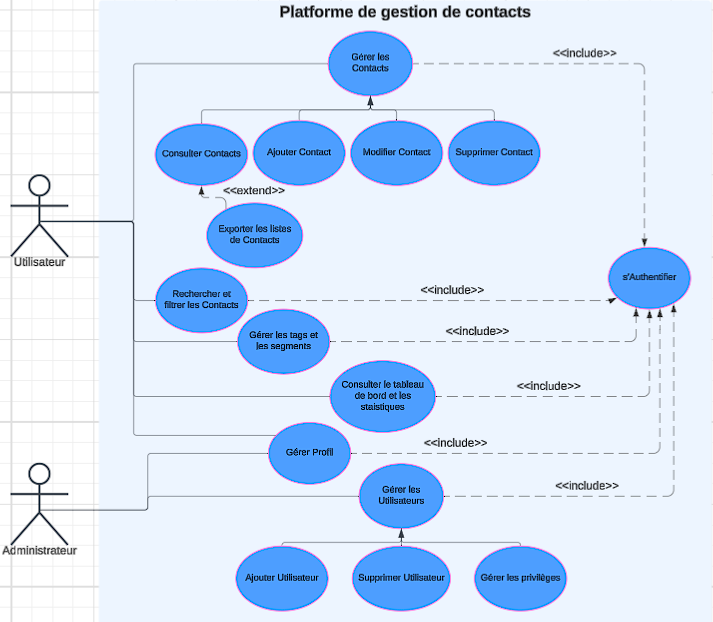
\includegraphics[width=0.6\textwidth]{images/diagramme_cas_utilisation.png}
\caption{Diagramme de cas d'utilisation du système}
\label{fig:dcu}
\end{figure}

Côté Utilisateur, les cas d'utilisation identifiés sont : s'authentifier, gérer son profil, gérer les contacts, exporter les listes, rechercher et filtrer, gérer les tags et les segments, et consulter le tableau de bord. L'Administrateur dispose d'un cas d'utilisation distinct, la gestion des comptes utilisateurs, sans accès aux fonctionnalités de l'Utilisateur.

\section{Besoins fonctionnels}

Les besoins fonctionnels précisent, pour chaque module, les fonctionnalités attendues de la plateforme. Ils sont présentés ci-dessous selon la logique de travail de l'application, puis résumés dans le tableau~\ref{tab:bf-synthese}.

\paragraph{Authentification et profil.}
Ce module sécurise l'accès à la plateforme : l'utilisateur s'authentifie par un identifiant et un mot de passe et peut gérer son profil.

\paragraph{Gestion des contacts.}
Ce module, au cœur de la plateforme, regroupe pour chaque contact des champs structurés (nom, organisation, pays, courriel).

\paragraph{Import.}
L'import alimente la base à partir de fichiers CSV ou Excel : les colonnes sont mises en correspondance, la validité des données est contrôlée et les doublons sont détectés, notamment par adresse électronique.

\paragraph{Numérisation OCR.}
La numérisation enrichit la base depuis des cartes de visite physiques : l'image est acquise, les informations extraites automatiquement, puis la fiche pré-remplie peut être corrigée avant enregistrement.

\paragraph{Recherche et segmentation.}
La recherche combine plusieurs critères (nom, pays, affiliation) pour retrouver rapidement un contact, tandis que la segmentation permet d'enregistrer et de réutiliser un ensemble de filtres afin de constituer des sous-ensembles de contacts.

\paragraph{Assistant IA.}
L'assistant permet d'interroger la base en langage naturel : les questions sont relayées à un service dédié qui consulte les contacts, en produit la synthèse et fournit des statistiques.

\paragraph{Tableau de bord.}
Le tableau de bord donne une vue de synthèse : des indicateurs récapitulent le nombre de contacts et leur répartition selon différents critères, avec une exploration interactive.

\paragraph{Export.}
L'export produit des fichiers CSV des listes de contacts, filtrées ou segmentées, avec la possibilité de personnaliser les champs inclus.

\paragraph{Administration.}
Ce module, réservé à l'administrateur, gouverne l'accès des utilisateurs à la plateforme par la gestion des comptes et l'attribution des rôles.

\begin{table}[H]
\centering
\small
\begin{tabularx}{\textwidth}{|l|X|}
\hline
\textbf{Module} & \textbf{Besoins clés} \\
\hline
Authentification et profil & Connexion et déconnexion sécurisées, gestion du profil, contrôle d'accès par rôle \\
\hline
Gestion des contacts & Création, consultation, modification et suppression des contacts (\acf{CRUD}), affichage de la liste \\
\hline
Import & Import CSV et Excel avec correspondance des colonnes, contrôle de validité des données, déduplication \\
\hline
Numérisation OCR & Acquisition d'une image de carte de visite, extraction automatique des informations, pré-remplissage et correction \\
\hline
Recherche et segmentation & Recherche multi-critères, filtrage, gestion des tags, segmentation \\
\hline
Assistant IA & Consultation de la base en langage naturel, synthèse d'un contact, statistiques \\
\hline
Tableau de bord & Indicateurs de synthèse, répartition des contacts par critères, exploration interactive \\
\hline
Export & Export des listes de contacts au format CSV, personnalisation des champs \\
\hline
Administration & Création et gestion des comptes utilisateurs, attribution des rôles, réservée à l'administrateur \\
\hline
\end{tabularx}
\caption{Besoins fonctionnels par module}
\label{tab:bf-synthese}
\end{table}

\section{Spécification des besoins non fonctionnels}

Outre les besoins fonctionnels, la plateforme doit satisfaire des exigences transverses de qualité, résumées dans le tableau~\ref{tab:bnf}.

\begin{table}[H]
\centering
\begin{tabularx}{\textwidth}{|l|l|X|}
\hline
\textbf{Catégorie} & \textbf{Besoin} & \textbf{Description} \\
\hline
Sécurité & Authentification et rôles & Accès sécurisé par mot de passe et contrôle d'accès par rôle \\
\hline
Sécurité & Protection des données & Accès aux contacts restreint aux utilisateurs authentifiés \\
\hline
Ergonomie & Interface conviviale & Interface web intuitive, responsive et facile à prendre en main \\
\hline
Performance & Temps de réponse & Réponses aux opérations courantes dans des délais acceptables \\
\hline
Maintenabilité & Architecture modulaire & Séparation claire des couches pour faciliter l'évolution \\
\hline
Déploiement & Disponibilité & Déploiement sur une infrastructure cloud accessible en ligne \\
\hline
\end{tabularx}
\caption{Besoins non fonctionnels}
\label{tab:bnf}
\end{table}

% ═══════════════════════════════════════════════════════════════════
% CHAPITRE 3 : CONCEPTION
% ═══════════════════════════════════════════════════════════════════

\chapter{Conception}

Le présent chapitre traduit les besoins spécifiés au chapitre 2 en une solution de conception : architecture logicielle et sa justification, modèle de classes, modèle de données, comportements dynamiques (diagrammes de séquence) et maquette de l'interface.

\section{Architecture logicielle}

\subsection{Choix d'une architecture trois-tiers}

La spécification des besoins a conduit à la mise en place d'une \textbf{architecture trois-tiers}, séparant la présentation, le traitement et la persistance (figure~\ref{fig:architecture}).

\begin{figure}[H]
\centering
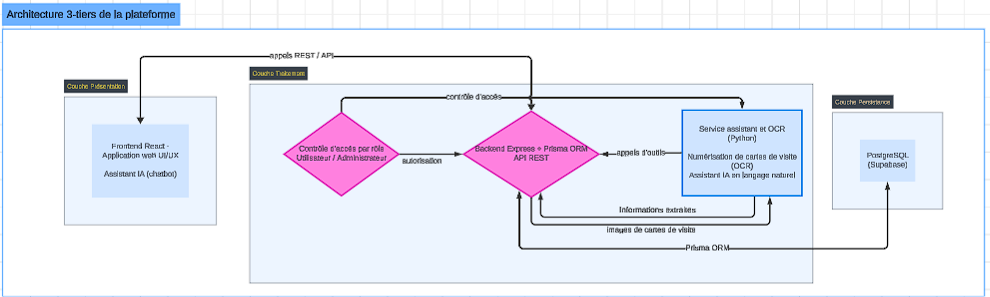
\includegraphics[width=1\textwidth]{images/architecture.png}
\caption{Architecture logicielle trois-tiers de la plateforme}
\label{fig:architecture}
\end{figure}

Ce choix répond à trois exigences posées au chapitre 2, détaillées dans le tableau~\ref{tab:exigences-archi}.

\begin{table}[H]
\centering
\small
\begin{tabularx}{\textwidth}{|l|X|}
\hline
\textbf{Plan} & \textbf{Justification} \\
\hline
Sécurité & Séparer le frontend du backend permet de n'exposer que des \acf{API} contrôlées et de protéger les accès à la base de données, jamais accessible directement par le client \\
\hline
Maintenabilité & La séparation des couches permet de faire évoluer chaque partie indépendamment sans impact sur les autres \\
\hline
Déploiement & Chaque couche peut être hébergée et dimensionnée sur une infrastructure adaptée \\
\hline
\end{tabularx}
\caption{Justification de l'architecture trois-tiers}
\label{tab:exigences-archi}
\end{table}

\subsection{Répartition des composants}

L'architecture distingue trois composants principaux, dont les rôles sont rassemblés dans le tableau~\ref{tab:composants}.

\begin{table}[H]
\centering
\small
\begin{tabularx}{\textwidth}{|l|X|}
\hline
\textbf{Composant} & \textbf{Rôle} \\
\hline
Frontend & Application web \acf{UI}/\acf{UX} chargée de l'affichage et de l'interaction : couche de présentation communiquant avec le backend par des appels \acf{REST}, et hébergeant le widget de l'assistant \\
\hline
Backend & Expose les \acf{API} \acf{REST} et porte la logique métier : gestion des contacts, de l'authentification et du contrôle d'accès, de l'import et de l'export. Il assure la persistance des données \\
\hline
Service assistant \& OCR & Service Python dédié portant d'une part la numérisation de cartes de visite (traitement d'images) et d'autre part l'assistant IA répondant en langage naturel, qui interroge le backend par appels d'outils \\
\hline
\end{tabularx}
\caption{Répartition des composants de l'architecture}
\label{tab:composants}
\end{table}

Le recours à un \textbf{service Python dédié} pour la numérisation OCR repose sur un écosystème de bibliothèques mature en Python (reconnaissance optique, prétraitement d'images, détection de zones textuelles). Ce même service héberge également l'\textbf{assistant IA} en langage naturel, qui sollicite le backend par des appels d'outils. Sa mise en œuvre est approfondie au chapitre de la réalisation.

\section{Modèle de classes}

Le modèle de classes de la plateforme est représenté à la figure~\ref{fig:classes}. Il traduit la structuration des entités du domaine identifiées lors de l'analyse des besoins.

\begin{figure}[H]
\centering
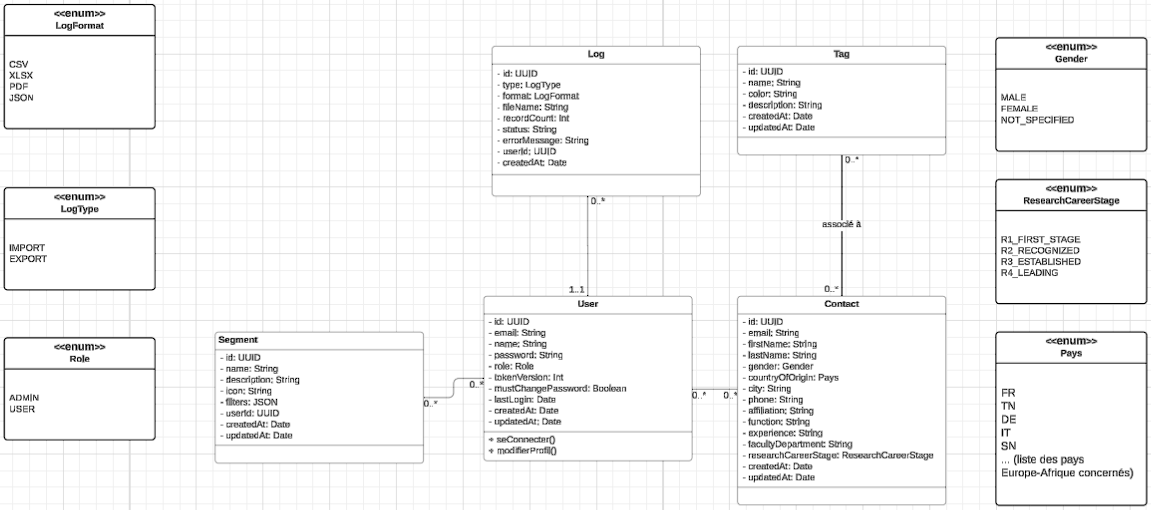
\includegraphics[width=1\textwidth]{images/diagramme_classes.png}
\caption{Diagramme de classes du système}
\label{fig:classes}
\end{figure}

La lecture de ce modèle met en évidence les relations clés du domaine, décrites dans le tableau~\ref{tab:entites}.

\begin{table}[H]
\centering
\small
\begin{tabularx}{\textwidth}{|l|X|}
\hline
\textbf{Entité} & \textbf{Rôle} \\
\hline
\texttt{User} & Modélise les comptes ; porte les attributs \texttt{role} (Utilisateur ou Administrateur) et \texttt{privilege}, support du contrôle d'accès \\
\hline
\texttt{Contact} & Représente les experts du réseau ; agrège l'ensemble des informations de la fiche (coordonnées, affiliation, fonction, stage de carrière) \\
\hline
\texttt{Tag} & Permet de catégoriser les contacts, un contact pouvant porter plusieurs tags et un tag s'appliquant à plusieurs contacts \\
\hline
\texttt{Segment} & Permet de conserver un ensemble de filtres sauvegardés afin de constituer des sous-ensembles de contacts \\
\hline
\end{tabularx}
\caption{Entités principales du domaine et leurs rôles}
\label{tab:entites}
\end{table}

Le choix de représenter le \textbf{stage de carrière} et le \textbf{genre} par des énumérations, plutôt que par des champs libres, contraint les valeurs possibles, évite les fautes de saisie et facilite le filtrage et les statistiques : une normalisation volontaire au service d'une exploitation fiable du réseau.

\section{Modèle de données}

Le modèle de données relationnel découle directement du modèle de classes et est implémenté avec l'\acf{ORM} Prisma sur une base PostgreSQL. Quelques contraintes en garantissent l'intégrité :
\begin{itemize}[leftmargin=*,itemsep=2pt]
  \item un identifiant de type UUID pour chaque entité.
  \item une adresse électronique unique pour les contacts, clé de déduplication lors des imports.
  \item la suppression en cascade des associations d'un contact ou d'un tag.
  \item des index sur les colonnes de filtres fréquents (pays d'origine du contact, associations de tags) pour accélérer la recherche et la segmentation.
\end{itemize}

\section{Diagrammes de séquence}

Pour illustrer les comportements dynamiques les plus significatifs, deux scénarios à forte valeur technique sont présentés : la consultation de la base via l'assistant IA et la numérisation d'une carte de visite.

Le premier scénario (figure~\ref{fig:seq-assistant}) illustre une consultation de la base en langage naturel. L'utilisateur pose sa question dans le widget de l'assistant. La requête est relayée au service assistant via le backend, qui la soumet au modèle de langage. Celui-ci sélectionne l'outil approprié parmi ceux exposés (recherche de contacts, synthèse d'un contact, statistiques). L'outil interroge alors le backend, dont les résultats reviennent au service, lequel formule une réponse affichée dans le widget.

\begin{figure}[H]
\centering
\includegraphics[width=0.8\textwidth]{images/sequence_assistant.png}
\caption{Diagramme de séquence : consultation de la base via l'assistant IA}
\label{fig:seq-assistant}
\end{figure}

Le deuxième scénario (figure~\ref{fig:seq-import}) déroule la numérisation d'une carte de visite. Après authentification, l'utilisateur transmet l'image au service OCR via le backend. Le service analyse l'image, en extrait les informations structurées et les renvoie au backend, qui pré-remplit la fiche de contact. Celle-ci est proposée à l'utilisateur pour validation avant enregistrement.

\begin{figure}[H]
\centering
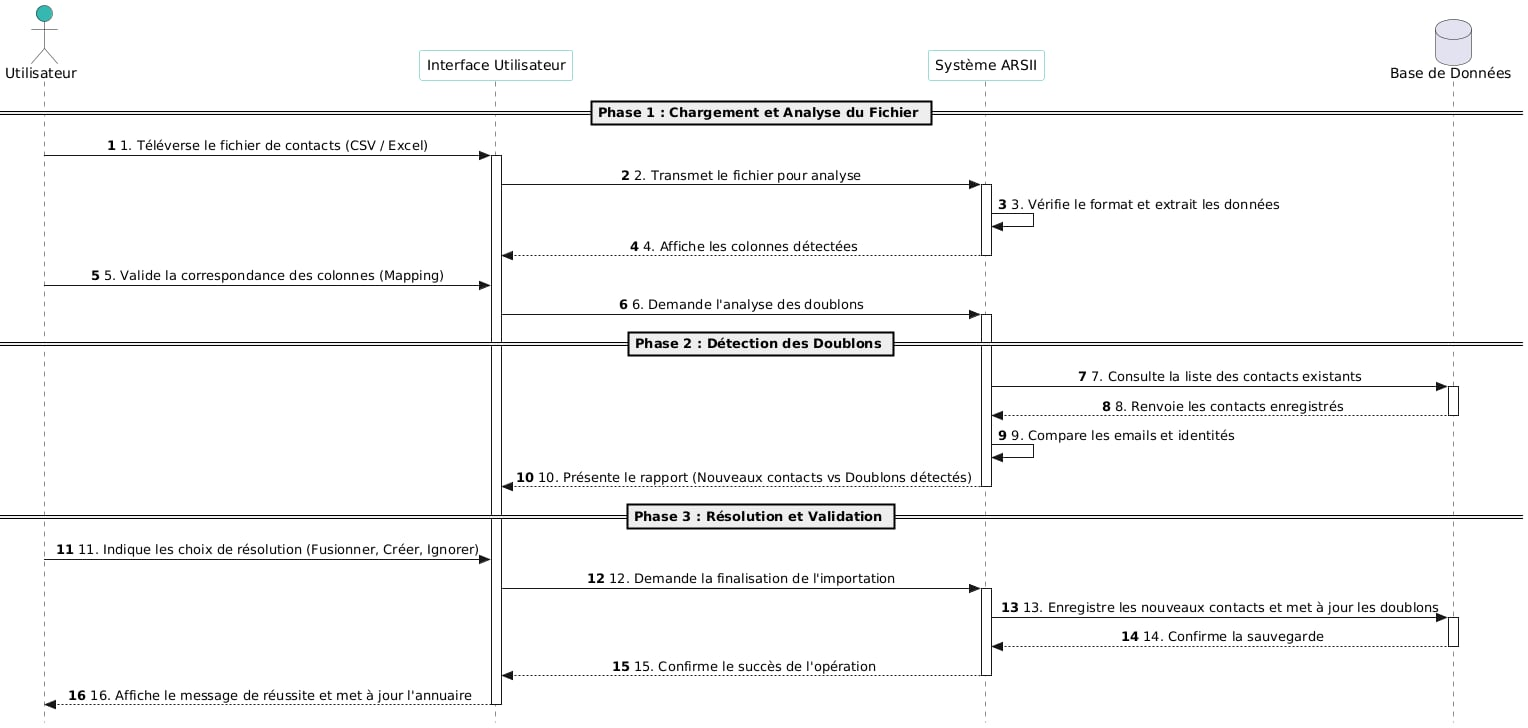
\includegraphics[width=0.8\textwidth]{images/sequence_import.png}
\caption{Diagramme de séquence : numérisation OCR d'une carte de visite}
\label{fig:seq-import}
\end{figure}

\section{Maquettage de l'interface}

La conception de l'interface a été menée à partir de maquettes établies au préalable, qui ont guidé le développement de chaque module et posent le cadre général de l'ergonomie et de la navigation.

\begin{figure}[H]
\centering
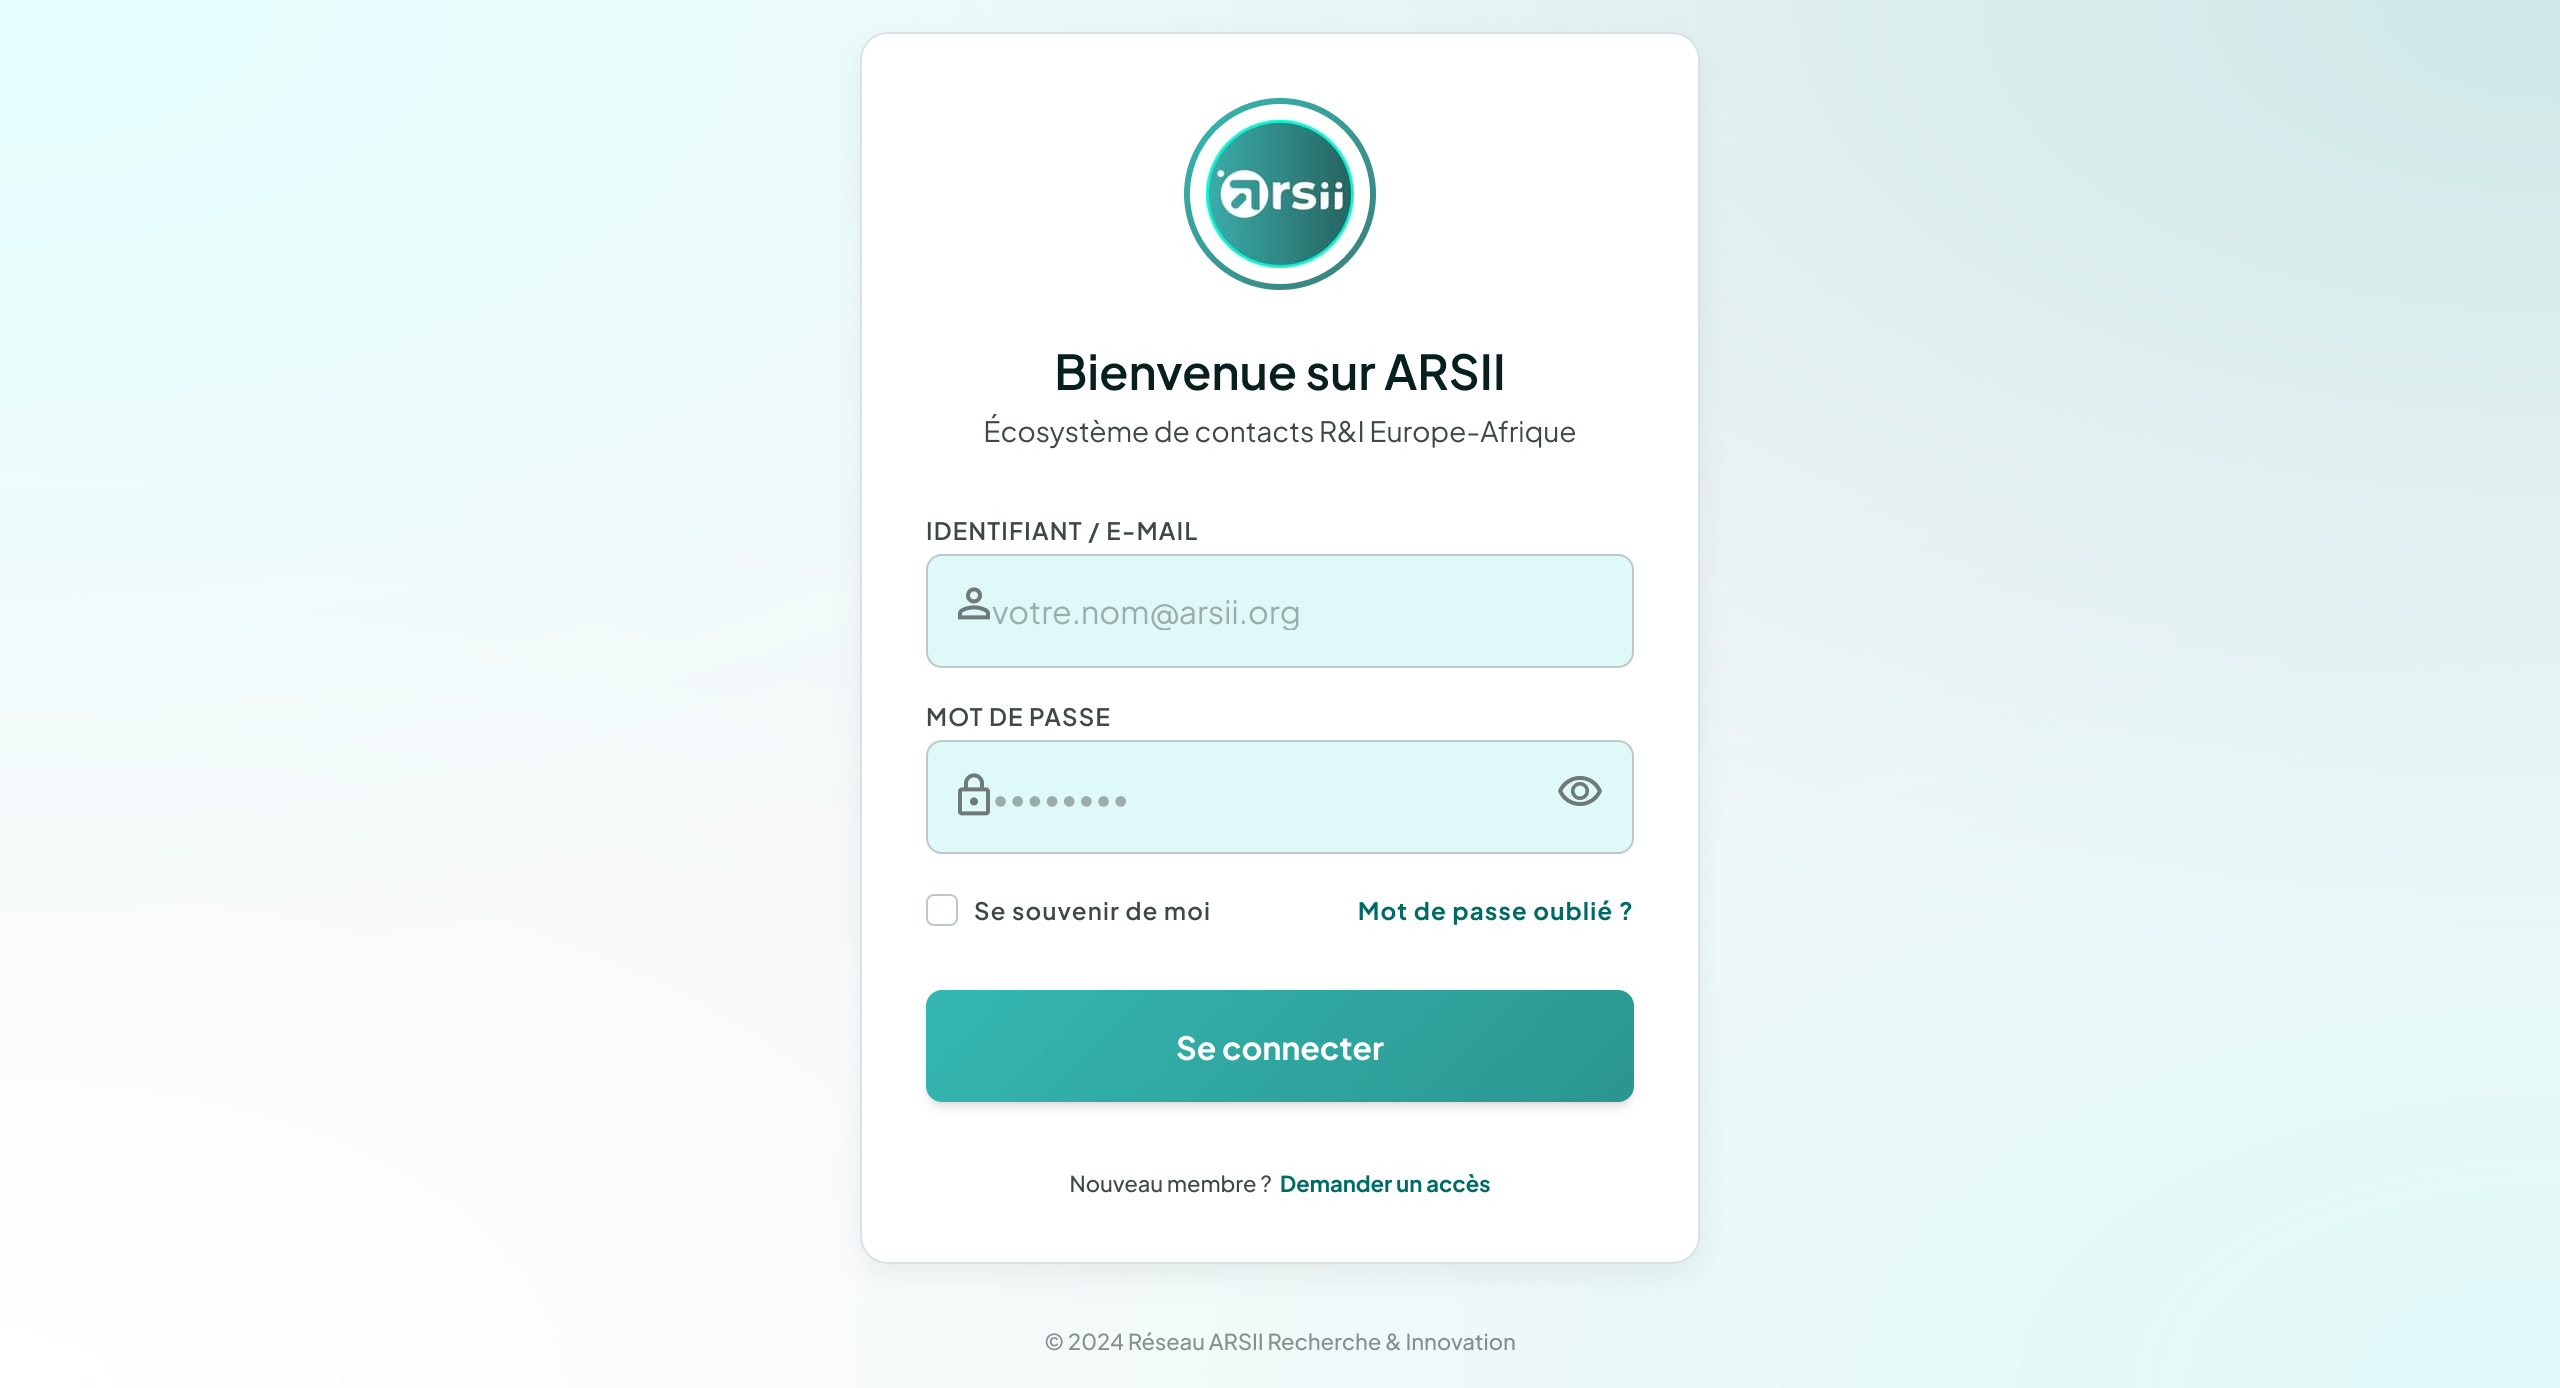
\includegraphics[width=0.8\textwidth]{images/maquette_connexion.png}
\caption{Maquette : écran de connexion}
\label{fig:maquette-connexion}
\end{figure}

\begin{figure}[H]
\centering
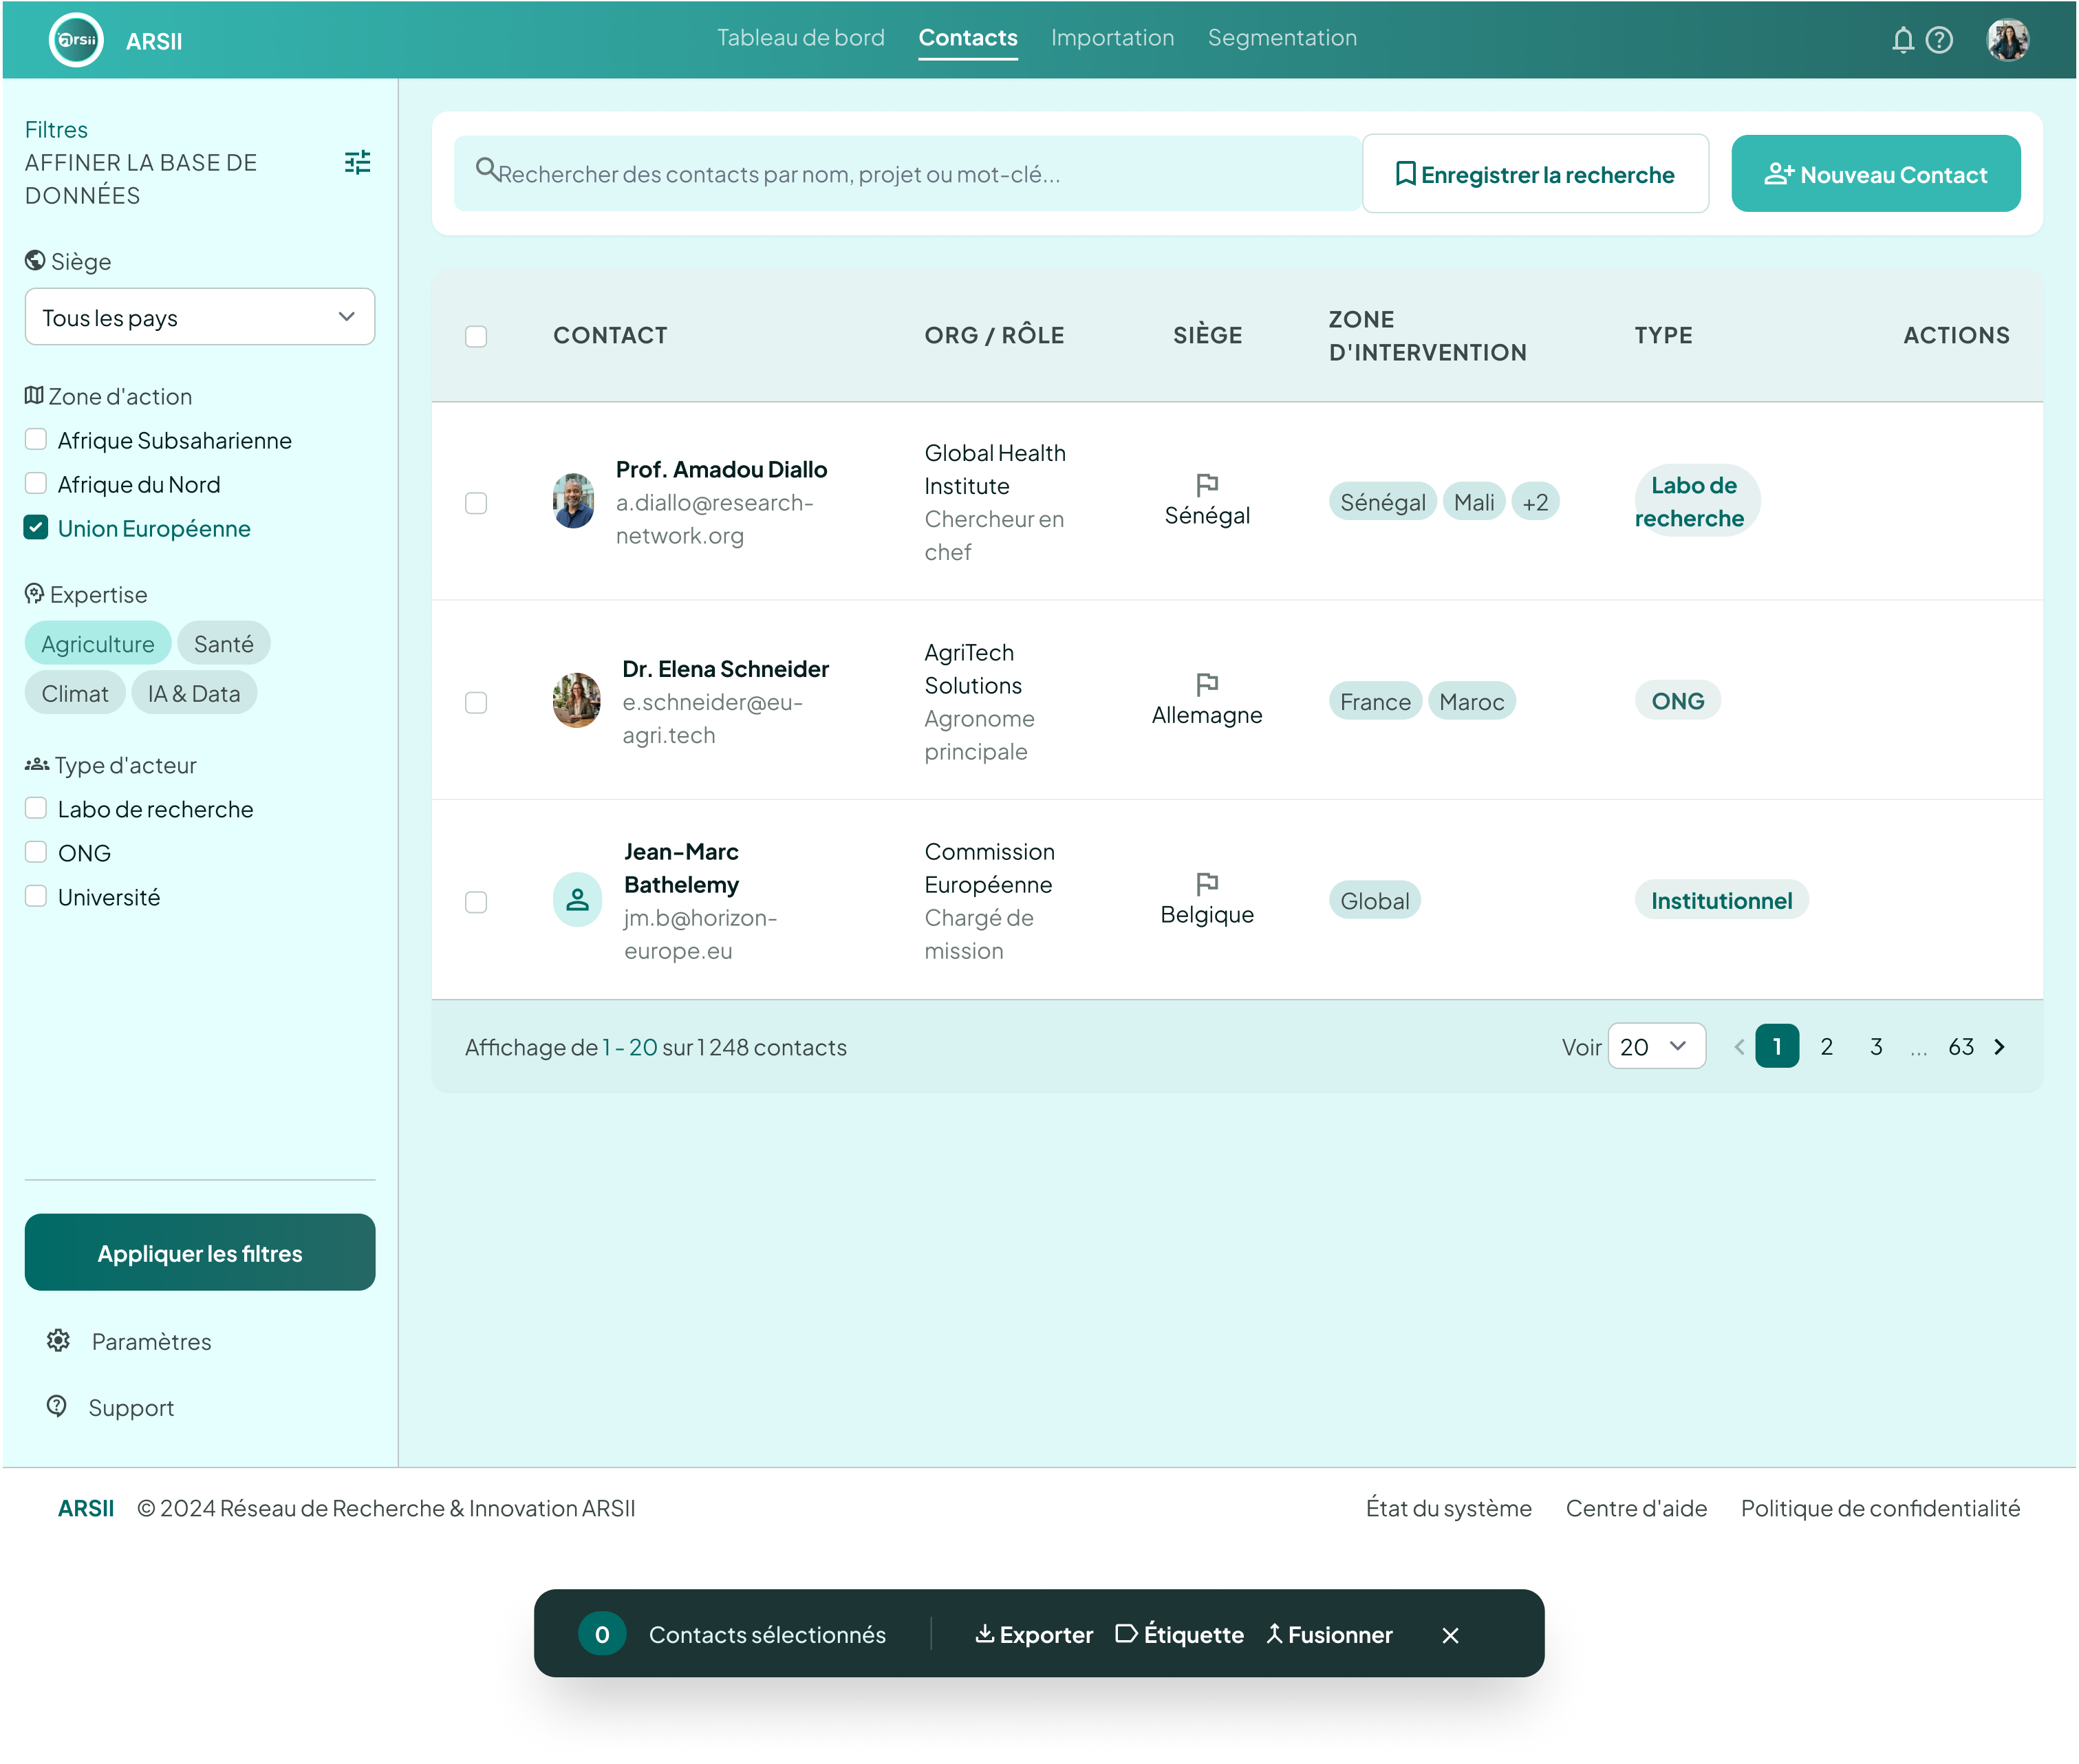
\includegraphics[width=0.9\textwidth]{images/maquette_liste_contacts.png}
\caption{Maquette : liste des contacts}
\label{fig:maquette-liste}
\end{figure}

\begin{figure}[H]
\centering
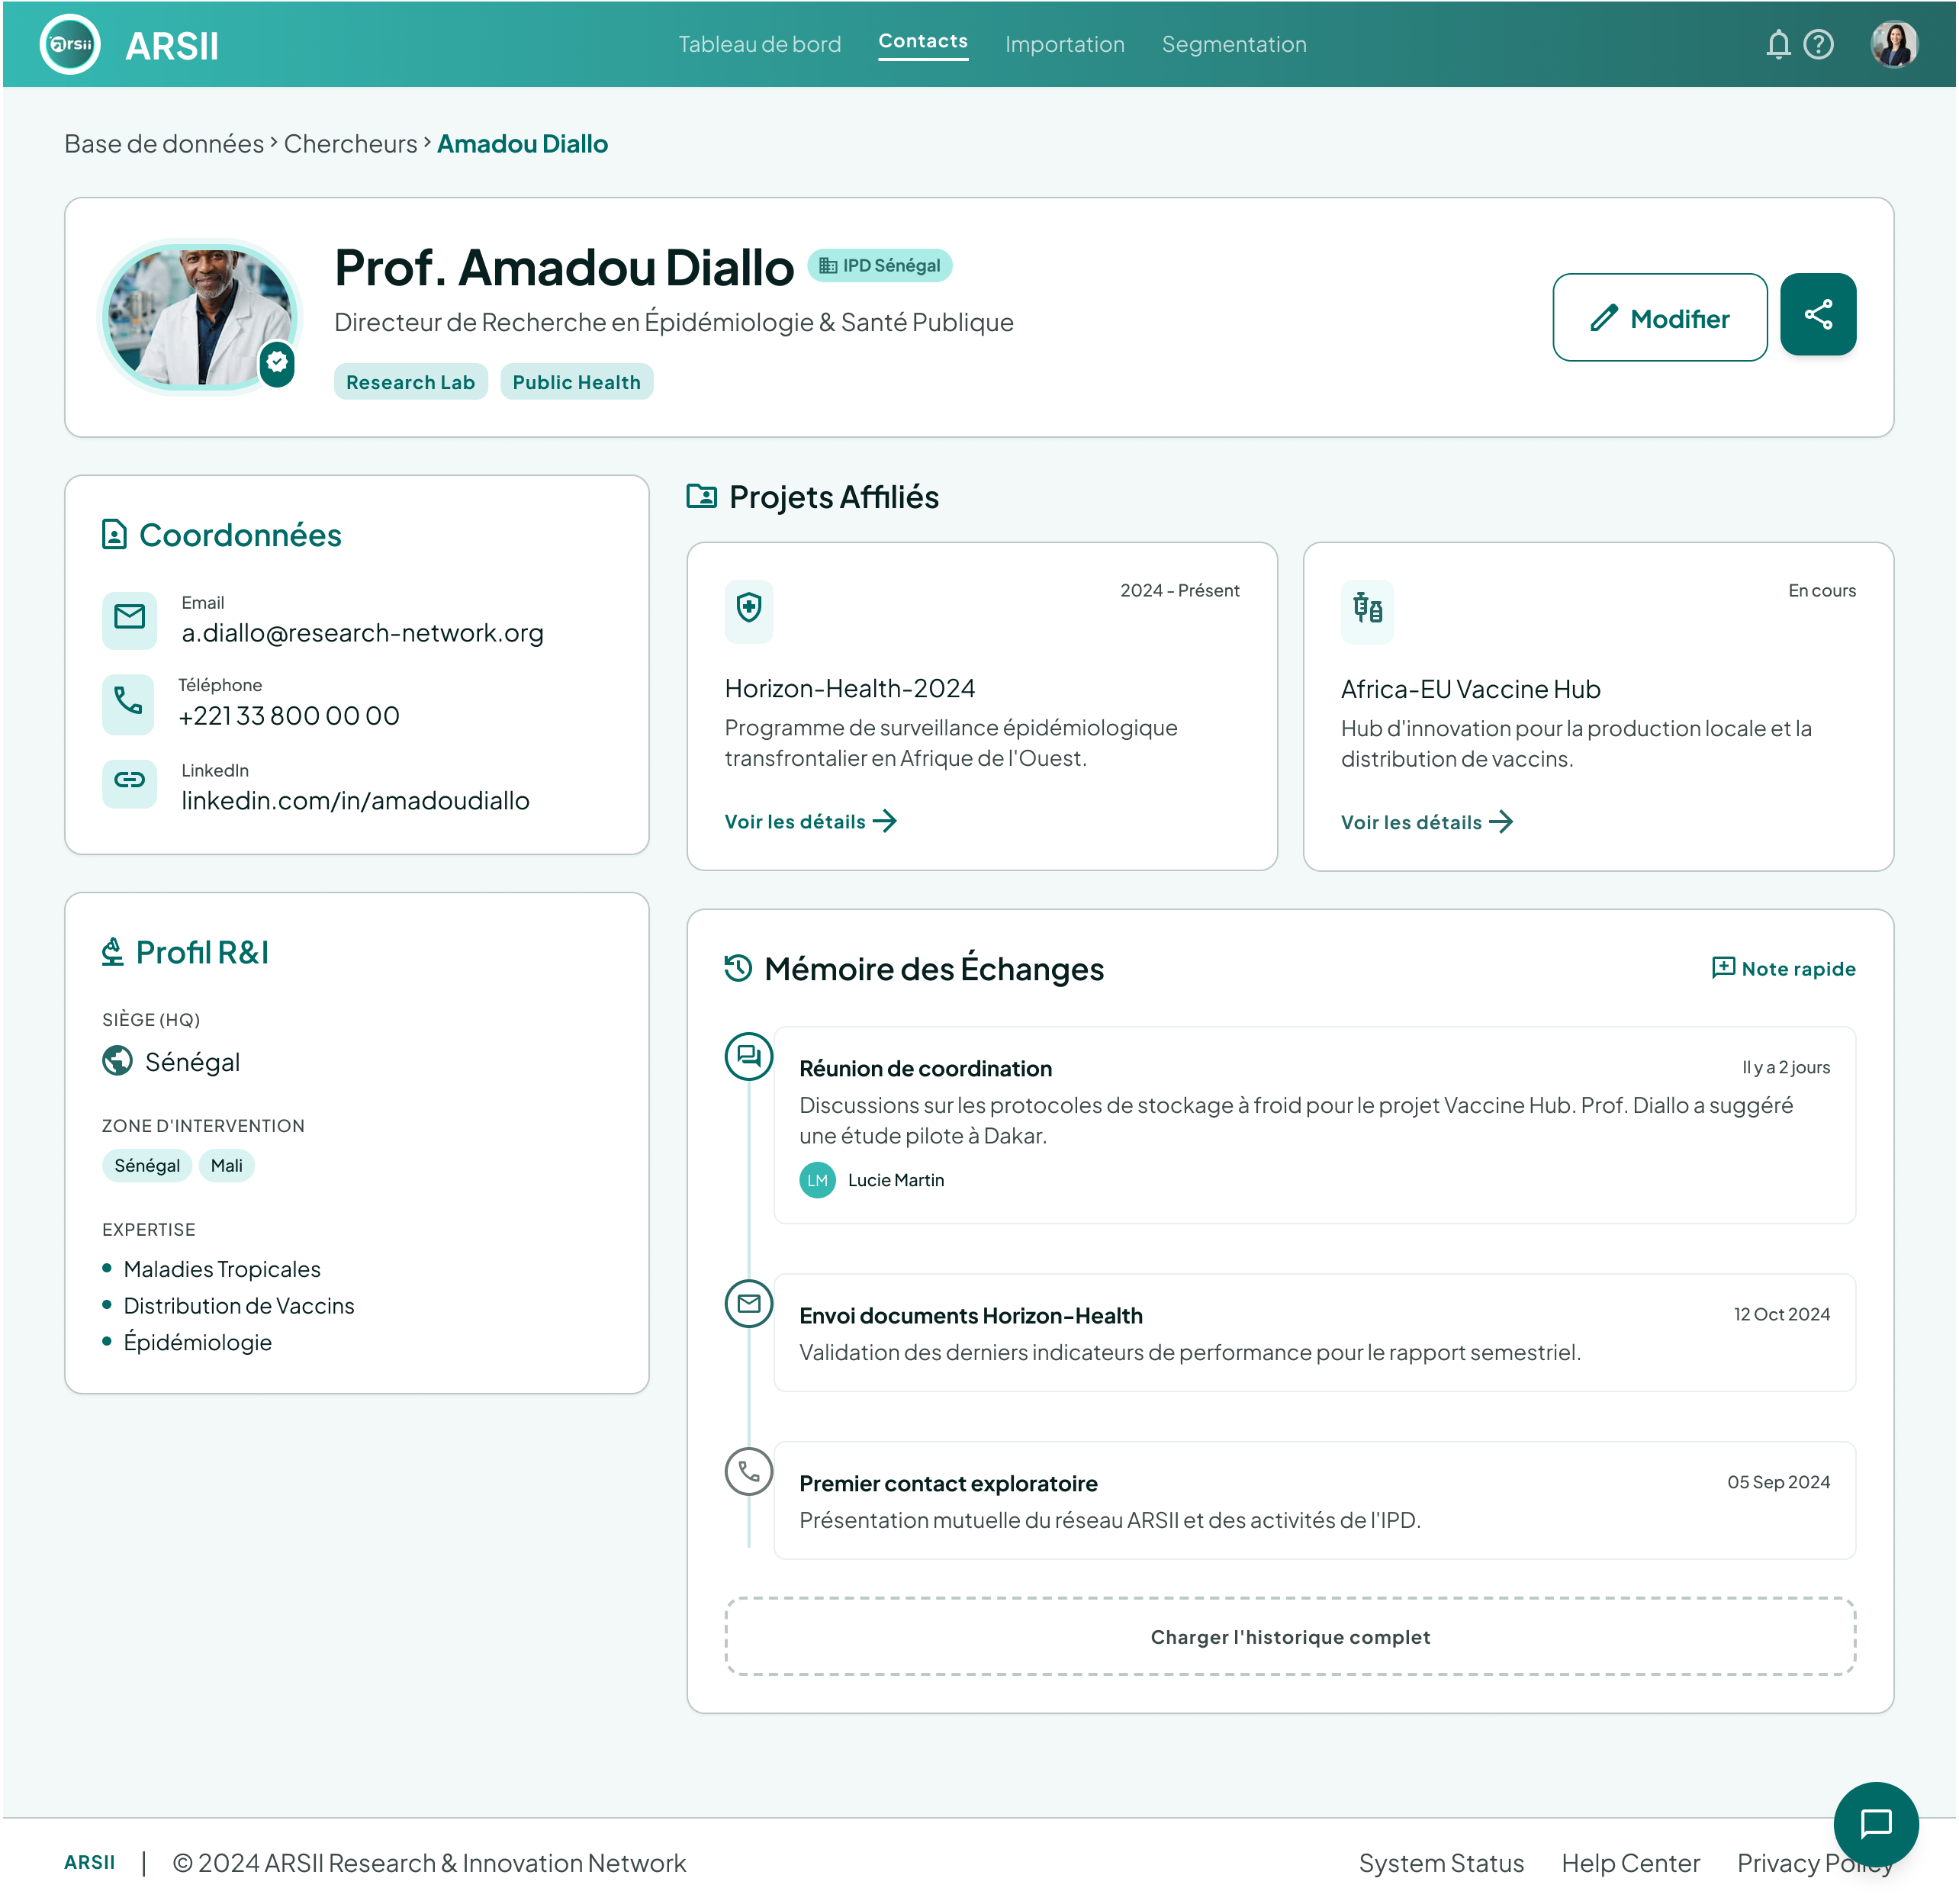
\includegraphics[width=0.9\textwidth]{images/maquette_fiche_contact.png}
\caption{Maquette : fiche contact}
\label{fig:maquette-fiche}
\end{figure}

\begin{figure}[H]
\centering
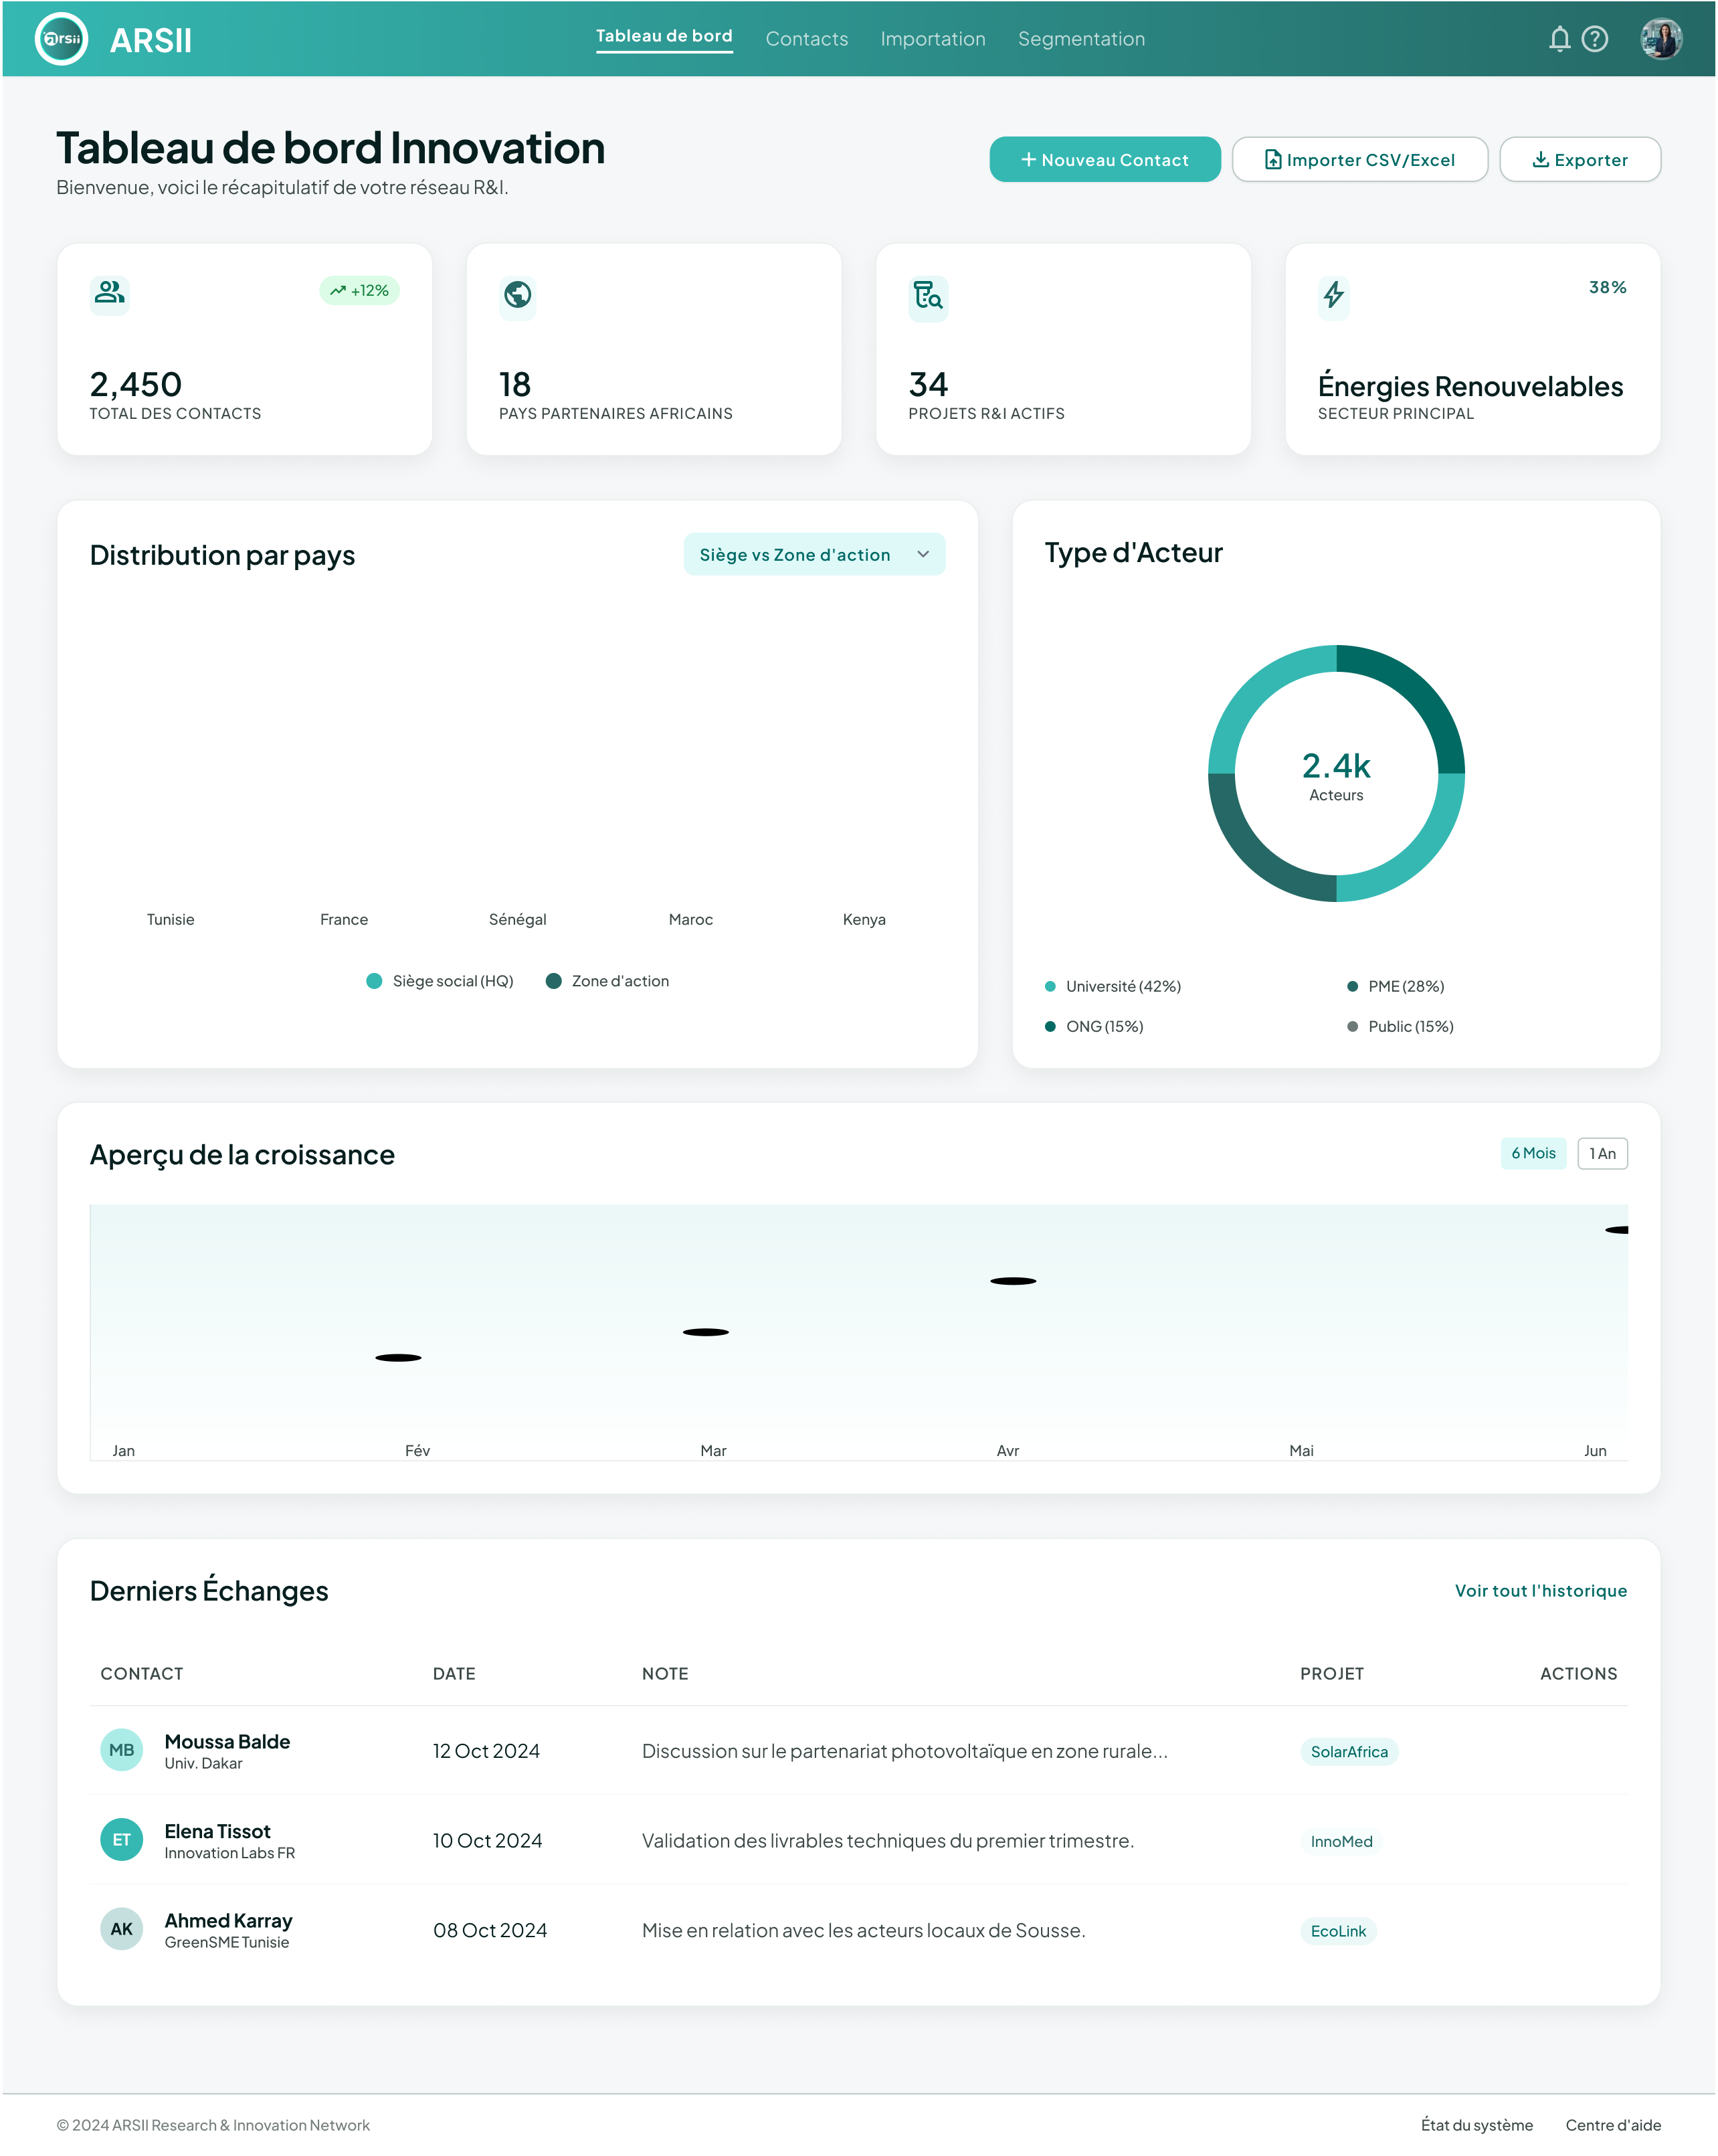
\includegraphics[width=0.9\textwidth]{images/maquette_dashboard.png}
\caption{Maquette : tableau de bord}
\label{fig:maquette-dashboard}
\end{figure}

Le choix du format de présentation vise une \textbf{prise en main rapide}, décliné par écran dans le tableau~\ref{tab:maquettes}.

\begin{table}[H]
\centering
\small
\begin{tabularx}{\textwidth}{|l|X|}
\hline
\textbf{Écran} & \textbf{Choix de conception} \\
\hline
Connexion & Écran minimal et centré \\
\hline
Liste des contacts & Tableau lisible, avec les actions principales accessibles \\
\hline
Fiche contact & Information regroupée de façon hiérarchisée \\
\hline
Tableau de bord & Indicateurs visuels de synthèse privilégiés \\
\hline
Assistant & Widget conversationnel accessible en permanence pour interroger la base \\
\hline
\end{tabularx}
\caption{Choix de conception pour les écrans principaux}
\label{tab:maquettes}
\end{table}

Ces choix ergonomiques répondent à l'exigence de convivialité des besoins non fonctionnels : l'interface se veut intuitive même pour un utilisateur non expérimenté.

Cette conception, de l'architecture au maquettage, fournit un cadre complet et cohérent pour la réalisation. Le chapitre suivant en détaille la mise en œuvre.

% ═══════════════════════════════════════════════════════════════════
% CHAPITRE 4 : RÉALISATION
% ═══════════════════════════════════════════════════════════════════

\chapter{Réalisation}

Ce chapitre décrit la mise en œuvre concrète de la solution conçue au chapitre 3. Après la présentation de l'environnement technique, il détaille la réalisation des modules, avec une attention particulière portée au module d'administration et au module de numérisation OCR, puis expose les difficultés techniques rencontrées et les solutions apportées.

\section{Environnement technique}

La réalisation s'appuie sur l'architecture trois-tiers définie au chapitre précédent. Le tableau~\ref{tab:techno} synthétise les technologies retenues pour chaque couche logicielle et le rôle de chacune ; le tableau~\ref{tab:deploiement} détaille la répartition des composants sur l'infrastructure cloud.

\begin{table}[H]\centering
\small
\begin{tabularx}{\textwidth}{|p{3cm}|l|X|}
\hline
\textbf{Couche} & \textbf{Technologie} & \textbf{Rôle} \\
\hline
Frontend & \begin{tabular}[t]{@{}l@{}} React + TypeScript \\ \raisebox{-0.5\height}{\includegraphics[height=3em]{images/logo_react}} \hspace{0.6em} \raisebox{-0.5\height}{\includegraphics[height=3em]{images/logo_typescript}} \vspace {0.4em}\end{tabular} & Interface utilisateur, composants, gestion des écrans, widget de l'assistant \\
\hline
Backend & \begin{tabular}[t]{@{}l@{}} Express (Node.js) \\ \raisebox{-0.5\height}{\includegraphics[height=3em]{images/logo_nodejs}} \end{tabular} & \acf{API} \ac{REST}, logique métier, authentification \\
\hline
Persistance & \begin{tabular}[t]{@{}l@{}} Prisma + PostgreSQL + Supabase \\ \raisebox{-0.4\height}{\includegraphics[height=3em]{images/logo_prisma}} \raisebox{-0.5\height}{\includegraphics[height=3.5em]{images/logo_postgresql}} \raisebox{-0.5\height}{\includegraphics[height=1em]{images/logo_supabase}} \end{tabular} & Accès aux données, schéma type-safe, persistance \\
\hline
Service assistant \& OCR & \begin{tabular}[t]{@{}l@{}} Python (FastAPI) \\ \raisebox{-0.5\height}{\includegraphics[height=3em]{images/logo_python}} \hspace{0.6em} \raisebox{-0.5\height}{\includegraphics[height=4.5em]{images/logo_fastapi}} \end{tabular} & Assistant IA en langage naturel et reconnaissance optique des cartes \\
\hline
\end{tabularx}
\caption{Couches logicielles et technologies retenues}
\label{tab:techno}
\end{table}

Le choix de \textbf{TypeScript} (frontend et backend) apporte un typage statique qui sécurise le développement. \textbf{Prisma} génère, à partir du schéma, un modèle de données type-safe garantissant la cohérence entre code et base. La base \textbf{PostgreSQL} est fournie par \textbf{Supabase}, choisi pour la simplicité d'approvisionnement d'une base cloud. Enfin, le \textbf{service Python} dédié porte d'une part le traitement OCR et d'autre part l'assistant IA en langage naturel, conformément à la justification du chapitre 3.

\begin{table}[H]
\centering
\small
\begin{tabularx}{\textwidth}{|p{3cm}|>{\raggedright\arraybackslash}p{3cm}|X|}
\hline
\textbf{Composant déployé} & \textbf{Plateforme} & \textbf{Rôle} \\
\hline
Frontend (React) & \raisebox{-\height}[0pt][\height]{\includegraphics[height=3em]{images/logo_vercel}} & Hébergement et diffusion de l'interface \\
\hline
Backend (Express) & \raisebox{-\height}[0pt][\height]{\includegraphics[height=5.5em]{images/logo_render}} & Hébergement de l'\acf{API} et de la logique métier \\
\hline
Service assistant \& OCR (Python) & \raisebox{-\height}[0pt][\height]{\includegraphics[height=5.5em]{images/logo_render}} & Hébergement du service d'assistant et de numérisation \\
\hline
\end{tabularx}
\caption{Déploiement des composants sur l'infrastructure cloud}
\label{tab:deploiement}
\end{table}

\section{Réalisation du module Administrateur}

Le module Administrateur met en œuvre la séparation des rôles définie lors de l'analyse. Il permet de créer, consulter, modifier et supprimer les comptes utilisateurs, une gestion réservée au rôle Administrateur. Son élément discriminant est l'\textbf{attribution du rôle} : à la création ou à la modification d'un compte, l'administrateur choisit entre les rôles Utilisateur et Administrateur, ce qui fixe les permissions accordées côté backend.

L'interface d'administration et les \acf{API} associées ne sont exposées qu'aux comptes Administrateur ; les comptes Utilisateur les voient masquées. La gestion des comptes reste ainsi entre les mains de l'acteur habilité (figure~\ref{fig:capture-admin}).

\begin{figure}[H]
\centering

\includegraphics[width=0.7\textwidth]{images/capture_admin.png}
\caption{Capture d'écran : interface d'administration des comptes utilisateurs}
\label{fig:capture-admin}
\end{figure}

\section{Réalisation du module de numérisation OCR}

Le module de numérisation OCR, le plus technique de la réalisation, met en œuvre le service Python dédié conçu au chapitre 3 et illustré par le diagramme de séquence de la figure~\ref{fig:seq-import}. Son fonctionnement suit un pipeline en plusieurs étapes.

\subsection{Pipeline de numérisation}

La numérisation d'une carte de visite suit un pipeline structuré :

\begin{enumerate}[leftmargin=*,itemsep=4pt]
  \item \textbf{Acquisition de l'image} : l'utilisateur importe ou capture une photographie de la carte depuis l'interface.
  \item \textbf{Traitement de l'image} : le service OCR prépare l'image (orientation, mise à l'échelle) pour améliorer la reconnaissance.
  \item \textbf{Extraction automatique} : le service analyse la carte et en extrait les informations structurées (nom, coordonnées, fonction, affiliation).
  \item \textbf{Pré-remplissage de la fiche} : les données extraites sont renvoyées au backend, qui pré-remplit la fiche de contact.
  \item \textbf{Correction et validation} : l'utilisateur vérifie et corrige les informations avant l'enregistrement définitif.
\end{enumerate}

La validation manuelle est essentielle car la reconnaissance peut être imparfaite selon la qualité de la carte, mais le pré-remplissage garantit un gain de temps important.

La figure~\ref{fig:capture-ocr} illustre le résultat de la numérisation, les informations extraites pré-remplissant la fiche de contact.

\begin{figure}[H]
\centering

\includegraphics[width=0.7\textwidth]{images/capture_ocr.png}
\caption{Capture d'écran : pré-remplissage de la fiche contact après numérisation OCR}
\label{fig:capture-ocr}
\end{figure}

\section{Réalisation de l'assistant IA}

L'assistant IA permet d'interroger le réseau en langage naturel via un widget accessible en permanence. Développé dans le service Python dédié, il s'appuie sur un modèle de langage et un mécanisme d'\textbf{appels d'outils} (\textit{function calling}). À la réception d'une question, il choisit l'outil adapté parmi ceux exposés par le backend (recherche de contacts, synthèse d'un contact, statistiques, journal d'import), puis formule une réponse à partir des résultats. Il exploite l'\acf{API} \acf{REST} existante sans exposer directement la base, ce qui préserve le contrôle d'accès.

\section{Autres modules réalisés}

Les autres modules du chapitre 2 ont également été réalisés conformément aux spécifications, comme le résume le tableau~\ref{tab:autres-modules}.

\begin{table}[H]
\centering
\small
\begin{tabularx}{\textwidth}{|l|X|}
\hline
\textbf{Module} & \textbf{Fonctionnalités réalisées} \\
\hline
Authentification et profil & Connexion sécurisée, déconnexion et gestion du profil, avec un contrôle d'accès par rôle servant de socle commun à toute l'application \\
\hline
Gestion des contacts & Création, consultation, modification et suppression des contacts, ainsi que l'affichage de la liste \\
\hline
Import & Alimentation de la base depuis des fichiers CSV ou Excel, avec contrôle de validité des données et gestion de la déduplication par adresse e-mail \\
\hline
Recherche et segmentation & Recherche avancée multi-critères, gestion des tags et segmentation en ensembles de filtres sauvegardés, permettant de regrouper et de catégoriser les contacts \\
\hline
Tableau de bord & Indicateurs de synthèse et répartition des contacts selon différents critères \\
\hline
Export & Export des listes de contacts, filtrées ou segmentées, au format CSV \\
\hline
Assistant IA & Consommation du \acf{API} REST sous forme d'outils : recherche multi-critères, synthèse d'un contact, statistiques, consultables en langage naturel via le widget \\
\hline
\end{tabularx}
\caption{Modules réalisés conformément aux spécifications}
\label{tab:autres-modules}
\end{table}

\section{Difficultés techniques rencontrées et solutions}

La réalisation a été marquée par une difficulté technique majeure : le problème de \textbf{connexion Prisma/Supabase}.

\subsection{Connexion Prisma/Supabase : diagnostic et résolution}

Lors de la mise en place de la persistance, la création des tables aboutissait, mais les requêtes échouaient. L'analyse a montré que la configuration de connexion entre Prisma et Supabase était en cause, en particulier la distinction entre l'accès direct et le pool de connexions. La solution a consisté à séparer la connexion servant aux migrations de celle des opérations courantes. La cohérence a ainsi été rétablie : les tables restent créées et les requêtes s'exécutent correctement.

Cette difficulté a souligné l'importance de comprendre comment un \acf{ORM} établit et réutilise ses connexions, et comment la configuration de l'infrastructure interagit avec le code applicatif.

% ═══════════════════════════════════════════════════════════════════
% CHAPITRE 5 : TESTS ET DÉPLOIEMENT
% ═══════════════════════════════════════════════════════════════════

\chapter{Tests et Déploiement}

Ce chapitre présente la stratégie de tests appliquée à la plateforme, son déploiement en production, puis une validation de la solution au regard des objectifs fixés au chapitre 1.

\section{Stratégie de tests}

La validation de la plateforme a reposé sur une stratégie de tests combinant plusieurs niveaux, adaptés à la taille du projet et à la nature du travail mené.

\subsection{Tests fonctionnels}

L'essentiel de la validation a consisté en des \textbf{tests fonctionnels manuels} portant sur les parcours métier de bout en bout. Chaque module a été parcouru selon des scénarios représentatifs :

\begin{itemize}[leftmargin=*,itemsep=3pt]
  \item connexion, déconnexion et gestion du profil ;
  \item création, consultation, modification et suppression d'un contact ;
  \item import d'un fichier CSV et d'un fichier Excel avec contrôle des données ;
  \item numérisation d'une carte de visite et validation du pré-remplissage ;
  \item recherche et filtrage multi-critères, et gestion des tags ;
  \item consultation du tableau de bord ;
  \item interrogation de la base via l'assistant IA en langage naturel ;
  \item export d'une liste de contacts ;
  \item côté administrateur, gestion des comptes et attribution des rôles.
\end{itemize}

Ces tests ont vérifié le comportement des fonctionnalités dans des conditions réalistes et ont conduit à des corrections, notamment sur la robustesse du traitement des fichiers importés et la validation des données extraites par l'\ac{OCR}.

\subsection{Analyse statique du code}

En complément, une \textbf{analyse statique} de la qualité du code a été intégrée au processus, menée avec \textbf{SonarQube}. Elle porte sur la détection de défauts potentiels (bugs, vulnérabilités, \textit{code smells}) et sur la maintenabilité du code. Servant de levier d'amélioration continue, les anomalies remontées ont été corrigées au fil du développement, fiabilisant le code avant sa mise en production.

\section{Déploiement}

Conformément à l'architecture trois-tiers, le déploiement répartit les composants sur une infrastructure cloud (figure~\ref{fig:deploiement}) : le \textbf{frontend} (React) est hébergé sur \textbf{Vercel}, le \textbf{backend Express} et le \textbf{service assistant \& OCR} (Python) chacun sur un \textbf{serveur Render} séparé, et la base PostgreSQL est fournie par \textbf{Supabase}.

\begin{figure}[H]
\centering

\includegraphics[width=0.7\textwidth]{images/deploiement.png}
\caption{Architecture de déploiement de la plateforme}
\label{fig:deploiement}
\end{figure}

Déployer le backend et le service assistant \& OCR sur \textbf{deux services Render distincts} suit la même logique que la conception : leurs profils de charge et cycles de vie diffèrent, et leur séparation permet de les faire évoluer, redéployer et dimensionner indépendamment. Le service assistant \& OCR, gourmand en calcul (modèle de langage et traitement d'images), est ainsi géré de façon isolée sans impact sur les \acf{API} métier.

\section{Bilan et validation par rapport aux objectifs}

Ce bilan reprend les objectifs énoncés au chapitre 1 et vérifie leur atteinte, comme le détaille le tableau~\ref{tab:bilan}.

\begin{table}[H]
\centering
\small
\begin{tabularx}{\textwidth}{|l|l|X|}
\hline
\textbf{Objectif} & \textbf{Statut} & \textbf{Vérification} \\
\hline
Centraliser & Atteint & La plateforme repose sur une base PostgreSQL unique, alimentée par la gestion des contacts et les imports, offrant une vision globale du réseau \\
\hline
Automatiser la saisie & Atteint & L'import CSV/Excel et la numérisation \ac{OCR}, validés par les tests fonctionnels, réduisent fortement la ressaisie manuelle \\
\hline
Organiser et exploiter & Atteint & La recherche avancée, le filtrage, la segmentation (ensembles de filtres sauvegardés), le tableau de bord et l'assistant IA permettent une exploitation fine du réseau \\
\hline
Sécuriser & Atteint & L'authentification sécurisée et la gestion des comptes réservée à l'administrateur sont opérationnelles et validées \\
\hline
\end{tabularx}
\caption{Bilan de l'atteinte des objectifs}
\label{tab:bilan}
\end{table}

Au terme de la réalisation, des tests et du déploiement, la plateforme répond aux objectifs initiaux et constitue une solution opérationnelle répondant à la problématique posée au chapitre 1. Les fonctionnalités livrées couvrent l'ensemble des besoins fonctionnels spécifiés au chapitre 2, et la solution est déployée et accessible sur une infrastructure en ligne.

% ═══════════════════════════════════════════════════════════════════
% CONCLUSION GÉNÉRALE
% ═══════════════════════════════════════════════════════════════════

\chapter*{Conclusion Générale}
\addcontentsline{toc}{chapter}{Conclusion Générale}

Ce rapport a rendu compte de l'ensemble du travail mené dans le cadre de ce stage d'été, de l'analyse des besoins à la validation d'une solution opérationnelle.

Le projet répondait à une problématique concrète de l'ARSII : la gestion dispersée et manuelle de ses contacts en Recherche et Innovation, qui empêchait une exploitation efficace de son réseau. Une plateforme web de gestion, d'organisation et d'enrichissement de bases de contacts a ainsi été analysée, conçue, réalisée, testée et déployée. Elle couvre l'ensemble des besoins identifiés : centralisation des contacts, automatisation de la saisie par import et numérisation OCR, exploitation fine du réseau par la recherche, la segmentation et le tableau de bord, et sécurisation de l'accès à deux rôles. Les tests fonctionnels et l'analyse statique ont validé le fonctionnement, et le déploiement cloud a rendu la plateforme accessible en ligne.

Sur le plan personnel, ce stage a permis d'acquérir une expérience concrète de développement d'une application web complète et du travail selon la méthodologie Agile/Scrum, de la spécification à la mise en production. La résolution d'une difficulté technique réelle (connexion Prisma/Supabase) a également développé la capacité d'investigation et de résolution de problèmes.

Plusieurs perspectives se dessinent : étendre la numérisation OCR à davantage de documents, affiner le modèle de rôles avec des permissions plus granulaires, et enrichir l'analyse du réseau par des indicateurs et visualisations supplémentaires dans le tableau de bord.


\end{document}
